%
%
\documentclass[11pt]{scrartcl}

% own geometry
%\usepackage[a4paper, left=3cm, right=3cm]{geometry}


\usepackage[ngerman]{babel} 
\usepackage[utf8]{inputenc} 
\usepackage[T1]{fontenc}
\usepackage{graphicx}
\usepackage{color}
\usepackage{xcolor}
%\usepackage{jurabib}
\usepackage{csquotes}
\usepackage{hyperref}
\usepackage[printonlyused]{acronym}
\usepackage{dirtree}
%fonts
\usepackage{helvet}
\renewcommand{\familydefault}{\sfdefault}
\fontfamily{phv}\selectfont

%\renewcommand*{\jbauthorfont}{\textsc}
\renewcommand*{\bibfnfont}{\normalfont}
\renewcommand*{\biblnfont}{\textsc}
%\renewcommand*{\samepageibidemname}{Ebd.}
\renewcommand*{\bibbtsep}{In: }
\renewcommand*{\bibjtsep}{In: }
\renewcommand*{\bibpldelim}{(}
\renewcommand*{\biburlprefix}{}
\renewcommand*{\biburlsuffix}{}

\makeatletter
\renewcommand*{\jbshorttitlefont}{%
\ifthenelse{%
\equal{\jb@@type}{article}%
\or
\equal{\jb@@type}{periodical}%
\or
\equal{\jb@@type}{incollection}%
}{%
\upshape%
}{%
\textit%
}%
}
\makeatother

\renewcommand*{\bibprdelim}{)}
\renewcommand*{\ajtsep}{}
\renewcommand*{\bpubaddr} { :}
\renewcommand*{\jbbtasep} { ; }
\renewcommand*{\jbbfsasep} { ; }
\renewcommand*{\jbbstasep} { ; }
\renewcommand*{\bibbtasep} { ; }
\renewcommand*{\bibbfsasep} { ; }
\renewcommand*{\bibbstasep} { ; } %between second and third author sep
\renewcommand*{\jbbtesep} { ; } %between two editors sep
\renewcommand*{\jbbfsesep} { ; } %between first and second editor sep
\renewcommand*{\jbbstesep} { ; } %between second and third editor sep
\renewcommand*{\bibbtesep} { ; } %between two editors sep
\renewcommand*{\bibbfsesep} { ; } %between first and second editor sep
\renewcommand*{\bibbstesep} { ; } %between second and third editor sep
\AddTo\bibsgerman{\def\editorsname{(Hrsg.)}}
\AddTo\bibsgerman{\def\editorname{(Hrsg.)}}
%\jurabibsetup{super, citefull=first,ibidem}
%\jurabibsetup{ibidem}
%\jurabibsetup{authorformat=citationreversed}
%\jurabibsetup{authorformat=reducedifibidem}
\jurabibsetup{biblikecite}
%\jurabibsetup{bibformat=ibidem}
%\jurabibsetup{pages=always}
\jbfirstcitepageranges
\AddTo\bibsgerman{\def\herename{hier}}
\jbuseidemhrule

\jurabibsetup{
  authorformat={smallcaps,year,and,citationreversed},
  titleformat={colonsep,all,italic},
  commabeforerest,
  see,
  dotafter=bibentry,
  ibidem=strict,
  biblikecite
}

\renewcommand*{\bibbtasep}{ und } %
\renewcommand*{\bibbfsasep}{, }   %
\renewcommand*{\bibbstasep}{ und }
\renewcommand*{\jbtitlefont}{}
\renewcommand*{\bibtfont}{}
\renewcommand*{\bibbtfont}{}
\renewcommand*{\bibjtfont}{}
\renewcommand*{\bibapifont}{}
\renewcommand*{\jbshorttitlefont}{}



	%
	% CITATIONS
	%
\newcommand{\book}[2]{\footnote{\cite[Vgl.][#2]{#1}}}
\newcommand{\bookwf}[2]{\cite[Vgl.][#2]{#1}}
\newcommand{\bookdir}[2]{\footnote{\cite[][#2]{#1}}}
\newcommand{\inetwf}[1]{\cite[Vgl.][\citefield{url}{#1}]{#1}}
\newcommand{\inetwfdir}[1]{\cite[][\citefield{url}{#1}]{#1}}
\newcommand{\inet}[1]{\footnote{\inetwf{#1}}}
\newcommand{\inetdir}[1]{\footnote{\cite[][\citefield{url}{#1}]{#1}}}
\newcommand{\innerref}[1]{\footnote{Vgl. auch Kapitel \ref{#1} dieser Arbeit, S. \pageref{#1}}}
\newcommand{\vgl}[2]{\cite[Vgl.][#2]{#1}}
\newcommand{\citeauthoryear}[1]{\citeauthor{#1} (\citeyear{#1})}
%\bibliographystyle{jurabib}
\usepackage[
	backend=biber,
	style=alphabetic,
	citestyle=alphabetic,
	sorting=nty,
	doi=true,url=true
]{biblatex}
\bibliography{bib/bib}

% setup of source code listings
\usepackage{listings}
%\usepackage{courier}
\usepackage{caption}
\lstset{
	basicstyle=\footnotesize\ttfamily,	% default font
	numbers=left,						% line numbers placement
	numberstyle=\tiny,					% line numbers style
	%stepnumber=2,						% line number padding
	numbersep=5pt,						% padding between line numbers and code
	tabsize=2,							% 
	extendedchars=true,         
	breaklines=true,						% line breaks 
	keywordstyle=\color{red},
	frame=b,
	stringstyle=\color{gray}\ttfamily,	% color of strings in code
	showspaces=false,					% visualize spaces
    showtabs=false,						% visualize tabs
    xleftmargin=17pt,
	framexleftmargin=17pt,
	framexrightmargin=5pt,
	framexbottommargin=4pt,
	showstringspaces=false				% visualize spaces in strings        
 }
 
 \lstloadlanguages{% Check docs for further languages ...
         C,
         C++,
         bash,
         HTML,
         Java,
         Clean % use this for CSS
 }

\setlength{\parindent}{0pt}
\setlength{\parskip}\medskipamount

\DeclareCaptionFont{white}{\color{white}}
\DeclareCaptionFormat{listing}{\colorbox{gray}{\parbox{\textwidth}{#1#2#3}}}
\captionsetup[lstlisting]{format=listing,labelfont=white,textfont=white}

% layout the caption ontop of code
\captionsetup[lstlisting]{format=listing,labelfont=white,textfont=white, singlelinecheck=false, margin=0pt, font={bf,footnotesize}}

% Headings
\usepackage{fancyhdr}
\renewcommand{\footrulewidth}{0.4pt}
\cfoot{}
\rfoot{\thepage}

% Document begins now
\begin{document}

\author{%
	Oliver Erxleben \small(\href{mailto:oliver.erxleben@hs-osnabrueck.de}{oliver.erxleben@hs-osnabrueck.de})\\%
	Albert Hoffmann \small(\href{mailto:albert.hoffmann@hs-osnabrueck.de}{albert.hoffmann@hs-osnabrueck.de})\\%
	\\%
	Hochschule Osnabr"uck \\%
	Ingenieurswissenschaften und Informatik \\%
	Informatik - Mobile und Verteilte Anwendungen\\
	Mensch-Maschine-Kommunikation - Wintersemester 2013/14 }

\title{
\includegraphics[scale=0.75,keepaspectratio]{img/hs_os.png}\linebreak \linebreak Entwicklung eines Usability-Test-Tools für Android}

\maketitle
\thispagestyle{empty}
\pagebreak
\thispagestyle{empty}
\tableofcontents

\listoffigures

\lstlistoflistings
\thispagestyle{empty}
\pagebreak

\thispagestyle{empty}

\begin{abstract}

\noindent\textbf{Zusammenfassung:}\\ \\
Die vorliegende Ausarbeitung wurde in \LaTeX verfasst und ist eine gemeinsame Arbeit von Albert Hoffmann und Oliver Erxleben an der Hochschule Osnabrück / University of Applied Sciences im Masterstudiengang Informatik - Mobile und Verteilte Anwendungen des Fachbereichs Ingenieurswissenschaften und Informatik für das Modul Mensch-Maschine-Kommunikation im Wintersemester 2013/14. Die Arbeit dokumentiert die Entwicklung einer Programmierbibliothek zum Test der Usability von Mobilanwendungen für das Android-Betriebssystem.\\ \\
Die Arbeit gliedert sich in verschiedene Teile.\\
%TODO: update Aufbau und Ablauf
\end{abstract}

\pagebreak
% set new page style

\pagestyle{fancy}
\setcounter{page}{1} 

% Einleitung 
\section{Motivation}
\label{motivation}

Mobile Anwendungen, sowie mobile Versionen einer Web-Site oder Web-Anwendung sind seit dem Aufkommen von Smartphones und Tablets im täglichen Leben unserer Gesellschaft verankert. Diese Anwendungen, allgemeinhin als \textit{Apps} bezeichnet, sollen uns im Alltag helfen, vernetzen, navigieren oder gar zerstreuen. Die Möglichkeiten der mobilen Hardware erweitern sich mit jeder Revision. Neue Programmierschnittstellen und präzisere Sensoren ermöglichen eine stetige Verbesserung und neue Nutzungsmöglichkeiten für mobile Endgeräte. 

Neben den Funktionen die durch Apps bereitgestellt werden, müssen diese aber auch leicht zu benutzen sein. Jede Funktion kann noch so hilfreich sein, wenn sie nur schlecht bedienbar ist. 

Das Thema \textit{Usability} spielt für die Software-Entwicklung eine immer größere Rolle. Eine Anwendung kann sich nur gut verkaufen, wenn sie auch bedienbar oder benutzerfreundlich ist, wenn sie sich "richtig anfühlt". Usability ist aber auch kein neues Thema im Software-Engineering. Seit Jahren beschäftigen sich Menschen mit der Verbesserung der Usability von Anwendungen.

Es werden Labor- oder Feldtests durchgeführt, Dienstleistungen werden angeboten und es werden Testprotokolle aufgezeichnet. Beispiele für solche Dienstleister sind: 

\begin{itemize}
    \item{http://www.userfeedbackhq.com/}
    \item{http://rapidusertests.com/}
    \item{http://www.usertesting.com/mobile}
\end{itemize}

Die Dienstleister erstellen mit Testsubjekten Anwendungstests und geben ein Feedback in Form von Video-, Audio- und Textmaterial. Dazu werden unterschiedliche Techniken eingesetzt. Zum Beispiel die Aufnahme des Smartphones über eine Helmkamera. 

Die gelisteten Dienste prüfen eine fertige App, einen Prototyp oder einen bestimmten Entwicklungsstand einer Anwendung. Usability-Tests sind aufwändig und teuer. Je nach Zielgruppe der Anwendung können hohe Kosten für einen Test entstehen. Es müssen geeignete Tester gefunden und es muss unter Umständen Hardware beschafft werden. Zudem kann das Testen sehr zeitintensiv werden. Weitere oder sehr hohe Kosten können entstehen, wenn der Usability-Test negativ ausfällt und viele Teile einer vielleicht fertigen Anwendung neu konzeptioniert und entwickelt werden müssen. 

Der aktuelle Stand der Technik zeigt das die Hardware des Endgeräts bereits alle technischen Vorraussetzungen erfüllt um Usability-Tests durchzuführen. So besitzen beispielweise fast alle Smartphones eine Frontkamera und Mikrofon womit Bild und Ton eines Testers aufgezeichnet werden kann. 

Wenn Usability-Tests bereits früh durchgeführt werden können, Funktionen zum Test von Usability bereitgestellt werden und kleinere Pakete der Software getestet werden, können schon früh und rechtzeitig Probleme bei der Usability gefunden und behoben werden.

Es stellt sich die Frage, wie Usability bereits während der Entwicklung getestet werden kann und wie eine Bibliothek, bzw. ein Framework, Funktionen zum Usability-Test bereitstellen kann. Welche Funktionen muss eine Bibliothek aufweisen um Usability zu testen? Diesen Fragen, sowie der Machbarkeit einer solchen Programmierbibliothek, widmet sich die vorliegende Ausarbeitungen. 

%TODO: Revision 1 - Korrektur?!


%example citings
%\cite{usabilityblog_eResult}

%\cite{usabilityblog_wasBeachten}

%\cite{usabilityEngineeringKompakt}
\pagebreak

\section{Testen von Usability}
\label{usability_testing}

Dieser Abschnitt stellt mögliche Vorgehen beim Testen von Usability vor, grenzt sie voneinander ab und bewertet sie für die Implementierung der Bibliothek. 

Die Anforderungen an das \textit{Mobile Web} und an \textit{Apps} unterscheiden sich stark von den klassischen Desktop-Anforderungen. Aufgrund der geringeren Displaygröße und Multitouch-Funktionalitäten in der Bedienung lösen neue Anforderungen die klassischen ab oder erweitern die vorhanden Anforderungen. 

\subsection{Testmethoden}

% TODO: Testarten, Methoden, Abgrenzung, .... Theorie und Transferleistung
\subsubsection{Formale Usability-Tests}

Nach dem Ablauf formaler Usability-Tests, kann eine Anwendung hinsichtlich Usability formativ und summativ evaluiert werden. Während die formative Evaluation die Verbesserung des zu prüfenden Systems zum Ziel hat, soll die summative Evaluation eine zusammenfassende Qualitätskontrolle sicherstellen. 
Der allgemeine Ablauf ist folgernder: es wird eine Testserie mit sog. Standardaufgaben erstelllt. 

\cite{usabilityblog_wasBeachten}

\cite{usabilityblog_eResult}
\pagebreak

\section{Anwendungsarchitektur}
\label{app_architecture}
Dieser Abschnitt beschreibt das implementierte System in der Gesamtheit. Das zu implementierende Werkzeug kann in zwei Bereiche gegliedert werden, dem Android-Client und dem HTTP-Server. 
Grundlegend handelt es sich hier um eine klassische Client-Server Architektur, bei der verschiedenartige Clients zum Einsatz kommen.

Der Server basiert auf Node.js.

Dadurch wird eine Abstraktion vom Betriebssystem erreicht.
Die zugrunde liegende Datenbank für die Persistenz ist MySQL, welches für verschiedene Plattformen verfügbar ist.
Für die Videokonvertierung wird AVLib benutzt, auch diese Software ist für verschiedene Plattformen verfügbar. Details zu den Serverkomponenten sind in Abschnitt \ref{server} zu finden.

Als Clients kommen einerseits die entwickelte Android-Bibliothek zum Einsatz, als auch handelsübliche Webbrowser.

Die einzelnen Komponenten und die Kommunikationsbeziehungen sind in Abbildung \ref{fig:architecture} dargestellt.

\begin{figure}[htb]
	\centering
	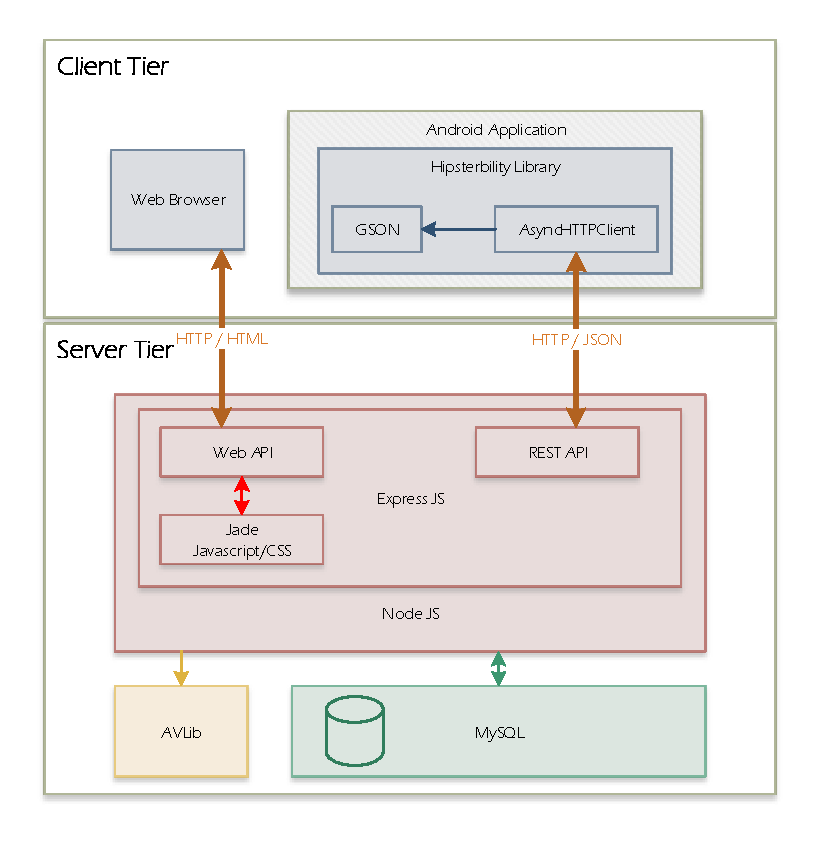
\includegraphics[width=0.75\linewidth]{img/architecture}
	\caption{hipsterbility Framework Architektur\label{fig:architecture}}
\end{figure}

\subsection{Client-Server-Kommunikation}
Nachfolgend werden die einzelnen Architekturkomponenten kurz betrachtet und in das Gesamtbild eingefügt. Hier liegt der Fokus auf der allgemeinen Kommunikationsbeziehung zwischen den einzelnen Elementen.


\subsubsection{Server}
Wie bereits erwähnt basiert der Server auf Node JS und nutzt Express JS als Webserver.
Dieser bietet zwei \ac{API}s an, eine Web API für Webbrowser und eine REST API für die reine Datenübertragung.

Die Kommunikation mit der MySQL Datenbank erfolgt über einen entsprechenden Datenbank Treiber.
Auch für AVLib existiert ein entsprechender Wrapper, welcher die Nutzung erleichtert.
Details zum Aufbau des Servers sind in Abschnitt \ref{server} zu finden.


\subsubsection{Webbrowser-Client}
Die Kommunikationsstruktur ist für den Webbrowser Client als reiner Online-Dienst ausgelegt.
Dies bedeutet, dass der Client die -- vom Server abgerufenen -- Daten nicht dauerhaft zwischenspeichern, sondern nur zur Darstellung und für die aktuelle Funktionserfüllung nutzen.
Für die abgerufenen Daten erfüllen der Browser nur die Funktion des \emph{Renderers}, da die Aufbereitung bereits vom Server vorgenommen wird.

Übertragen werden fertige HTML-Seiten mit Javascript und \ac{CSS}.
Diese werden mit \emph{Jade}-Skripten erstellt (siehe Abschnitt \ref{sec:node-mudules}) und über die Web API des Webservers ausgeliefert.
Eine ausführliche Erläuterung des webbasierten Verwaltungstools \ref{sec:web_verwaltung}.


\subsubsection{Android-Client}
Bei der Android Bibliothek handelt es sich um eine Hybrid-Online Lösung.
Zu Beginn werden Daten vom Server abgerufen, nach der initialen Kommunikation speichert der Client Daten zwischen, die erst am Ende der Ausführung an den Server übertragen werden.
Zwischen diesen beiden Kommunikationsbeziehungen benötigt der Client keine dauerhafte Serververbindung.

Der Android-Client kann seine Funktion jedoch nicht ohne Serververbindung aufnehmen, diese wird an zwei Zeitpunkten, wie beschrieben, zwingend benötigt.
Der Datenaustausch zwischen Client und Server erfolgt über eine REST API, welche in Abschnitt \ref{sec: api} genauer beschrieben wird.

Die Daten werden in der \ac{JSON} Notation im HTML-Body vom Server abgerufen, bzw. als MultiPart Daten über HTTP vom Client zum Server übertragen.
Eine detaillierte Beschreibung des Android-Clients erfolgt in Abschnitt \ref{sec:android_client}.
\pagebreak

\section{Server}
\label{server}
Wie in Abschnitt \ref{app_architecture} beschrieben, müssen die aufgezeichneten Daten der Clientbibliothek weiter verarbeitet werden. % nochmal etwas genauer

Im Folgenden werden die zwei serverseitigen Komponenten, Datenbank und HTTP-Server, vorgestellt. 

%TODO: footnote ++ update

%TODO: subsection title ?!
\subsection{Virtuelle Maschine}

\subsubsection{Konfiguration}

Als Betriebssystem für den Server dient ein Debian in der Version 7.0. Der Maschine wurde 1 Prozessorkern und 512 MB RAM zugewiesen. Änderungen können im Vagrantfile, siehe Abschnitt \ref{vagrant}, oder der Virtual Box-Konfiguration vorgenommen werden.

Weitere Softwarequellen, welche installiert wurden, sind: 
\begin{description}
	\item[openSSH Server] 
	Dieser 
\end{description}


\subsubsection{Ordnerstruktur}
% TODO positioning, sizing
\dirtree{%
 .1 /serverside.
 .2 classes.
 .2 controllers.
 	.3 api.
 		.4 audio.js.
 		.4 captures.js.
 		.4 log.js.
 		.4 sessions.js.
 		.4 tasks.js.
 		.4 todos.js.
 		.4 videos.js.
 	.3 backend.js.
 	.3 frontend.js.
 .2 node\_modules.
 .2 public.
 	.3 css.
 		.4 plugins.
 		.4 bootstrap.min.css.
 		.4 bootstrap-theme.min.css.
 		.4 sb-admin.css.
 		.4 style.css.
 		.4 video-js.min.css.
 	.3 fonts.
 	.3 img.
 	.3 js.
 .2 uploads.
 .2 views.
}
\subsubsection{Vagrant}
\label{vagrant}
Um die Bereitstellung der Serverumgebung zu vereinfachen wurde die virtuelle Maschine mittels Vagrant\footnote{Vagrant: http://www.vagrantup.com/} konfiguriert. Vagrant ist ein Kommandozeilenwerkzeug um schnell reproduzierbare Entwicklungsumgebungen zu schaffen und diese später zu verteilen oder zu exportieren. Dabei wird Virtual Box als Virtualisierungssoftware eingesetzt. Aber auch VMware wird unterstützt. 

Die eigene VM wird mittels einer VM-Schablone (die eigentliche VM) und einer Konfigurationsdatei geladen, die alle Eigenschaften der VM bereithält, zum Beispiel Portweiterleitungen. Die Schablone kann demnach bereits einige Standardsoftwarepakete beinhalten. 

Auf dem Host-System können die gewohnten Entwicklungswerkzeuge eingesetzt werden, da der Ordner, indem Vagrant konfiguriert wurd, mit dem Ordner /Vagrant auf dem Gast-System synchronisiert wird. 

Auch die Entwicklung von Software mittels einer Vagrant VM ergibt einen gut zu bedienenden Arbeitsfluss. So ist es beispielsweise möglich mittels \textbf{vagrant up} und \textbf{vagrant ssh} die Maschine zu starten und darauf zu verbinden, ohne dabei extra overhead, wie zum Beispiel Fenster, zu erzeugen. Die SSH-Credentials folgen dem \textit{Convention over Configuration}-Paradigma. Username, sowie Passwort lauten standardmäßig vagrant. 


\subsection{Datenbank}

Zur persistenten Speicherung der Nutzdaten wird MySQL verwendet. MySQL bietet sich an, da es Verbreitung und Sicherheit bietet, sowie von Oracle als kommerzielles, wie auch Open Source-Derivat entwickelt wird. Das Projekt nutzt die Community-Server-Edition. 
%TODO: Links in footnotes

\subsubsection{Datenbank-Modell}
Das Datenbankmodell wurde mit Hilfe des MySQL Workbench erstellt. Die Abbildung \ref{figure-db-model} zeigt das Ergebnis.
\begin{figure}[h!]
	\centering
	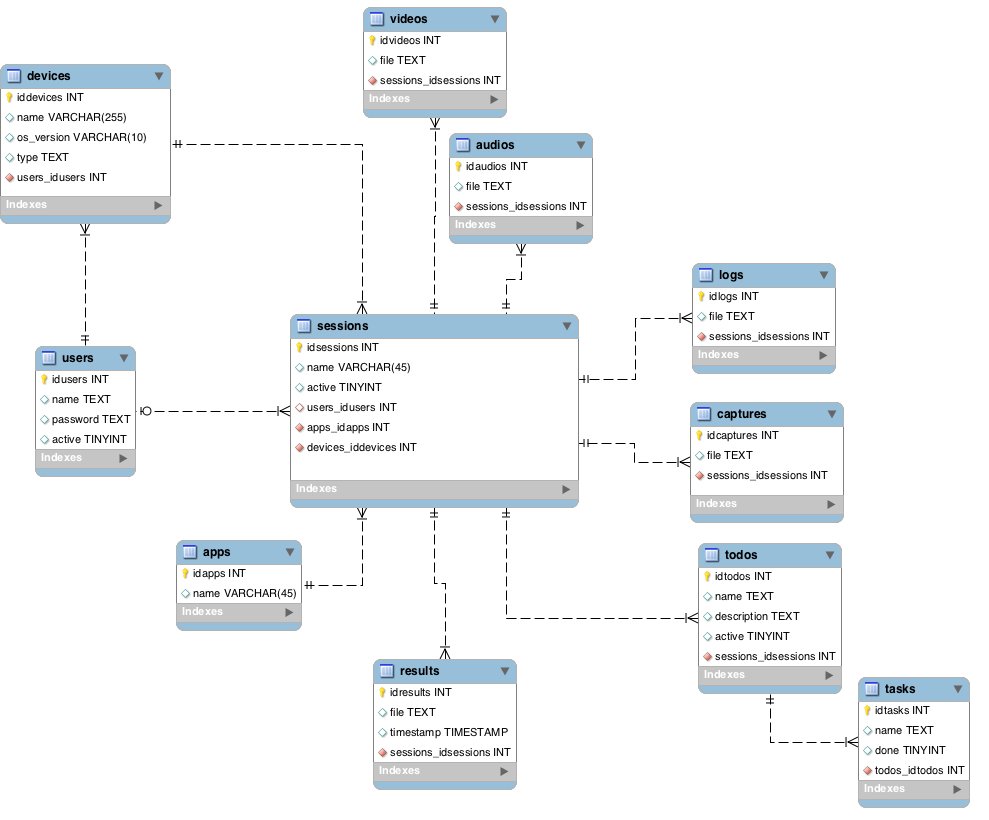
\includegraphics[width=\linewidth,keepaspectratio]{img/db_model.png}
	\caption{Datenbank Modell}
	\label{figure-db-model}
\end{figure}


\subsection{NodeJS HTTP-Server und Middleware}
Die serverseitige Logik wurde mit NodeJS und dem ExpressJS-Framework umgesetzt. Folglich wurde serverseitig Javascript eingsetzt. Javascript eigenet sich sehr für Programmierschnittstellen und HTTP-Anfragen. Nicht nur, da Javascript aus dem Web nicht mehr wegzudenken ist, sondern auch da es komplett asynchron programmiert werden kann. 

Das Express-Framework stellt die grundlegenden Funktionen eines Web-, bzw. HTTP-Servers bereit. Ein minimaler HTTP-Server ist im Listing \ref{minimal_node_http_server} zu sehen. 

\begin{lstlisting}[label=minimal_node_http_server,language=Java, caption=Minimaler Node-HTTP-Server]
/**
 * Module dependencies.
 */
var express = require('express');
var routes = require('./routes');
var http = require('http');
var path = require('path');
var app = express();

// environments config
app.set('port', process.env.PORT || 3000);
app.set('views', path.join(__dirname, 'views'));
app.set('view engine', 'ejs');
app.use(express.favicon());
app.use(express.logger('dev'));
app.use(express.json());
app.use(express.urlencoded());
app.use(express.methodOverride());
app.use(app.router);
app.use(express.static(path.join(__dirname, 'public')));

// simple test route
app.get('/ping', routes.pong);


// server take off
http.createServer(app).listen(app.get('port'), function(){
  console.log('Express server listening on port ' + app.get('port'));
});
\end{lstlisting}

\subsubsection{APIs}

\subsection{Videoproduktion}

Zur Erstellung der Zwischenergebnisse und des Endergebnisses wird die Open Source-Bibliothek \emph{libav}\footnote{} verwendet. Genauer wird die darin enthaltene Software \emph{avconv} genutzt um die Bilder und Videos zusammenzufügen. 

\pagebreak

\section{Android-Client\label{sec:android_client}}

In diesem Abschnitt wird die Entwicklung der Android-Bibliothek beschrieben. 
Zur Entwicklung wurde die plattformübergreifende IDE \emph{IntelliJ Idea}\footnote{IntelliJ Idea: \url{http://www.jetbrains.com/idea/}} verwendet.

Alternativ kann auch die offizielle Android \ac{IDE}, \emph{Android Studio}\footnote{Android Studio: \url{http://developer.android.com/sdk/installing/studio.html}}, verwendet werden, welche auf der \emph{Community Edition} von \emph{IntelliJ Idea} basiert, zum aktuellen Zeitpunkt jedoch nur in einer \emph{early access preview} verfügbar ist.
Die Projektdateien sind untereinander kompatibel.

Für UML-Diagramme wird die quelloffene, Eclipse basierte, Modellierungssoftware \emph{modelio}\footnote{modelio: \url{http://www.modelio.org/}} genutzt.

Screenshots und Anleitungen beziehen sich diesbezüglich auf diese Software. 
Konfigurationen und Einstellungen können sich zu anderen IDEs unterscheiden.
Die Quellen zu den Projekten befinden sich im Github-Repository im Unterordner \texttt{client}.

Als Hilfen für die Implementierung dienten hauptsächlich das Buch \citetitle{android4} von \citeauthor*{android4}, sowie einige Tutorials von \citeauthor*{androidvogella}\footnote{\citeauthor*{androidvogella}: \url{http://www.vogella.com/}}.
Außerdem wurden für spezielle Probleme Lösungen, Antworten und Quelltextauszüge von der Frage-Antwort-Website StackOverflow\footnote{StackOverflow: \url{http://stackoverflow.com/}} genutzt.
Diese sind in den Kommentaren in den Quelltexten der jeweiligen Klassen vermerkt.


\subsection{Ziele der Implementierung}
Bei der Konzeption und Entwicklung der Android Bibliothek wurden mehrere Ziele verfolgt.
Das Hauptziel ist die Erstellung einer Bibliothek, die sich leicht in Anwendungen integrieren lässt und die Funktionen aufwändiger Mobilgeräte-Usability-Testaufbauten mit externen Kameras, Mikrofonen etc. ersetzt.
Dazu sollen die technischen Möglichkeiten moderner Endgeräte genutzt werden.
Viele Smartphones und Tablets verfügen über eine Frontkamera für Videotelefonie, ein eingebautes, hochempfindliches, Mikrofon für (Freisprech-)Telefonie und Mehrkernprozessoren für Multitasking.

Diese Eigenschaften sollen genutzt werden um klobige Testaufbauten zu ersetzen. 
Deren Funktionalität besteht meist aus dem Aufzeichnen von Mimik und Sprache der Testperson, sowie Inhalt des Bildschirms und Interaktion mit dem Endgerät bzw. der Applikation.
Unter der Prämisse, dass moderne Smartphones und Tablets die nötigen Hard- und Softwarevoraussetzungen erfüllen soll nun eine Software-Lösung implementiert werden, um die zuvor genannten Funktionen abzubilden.

\pagebreak

\subsection{Verwendete Bibliotheken von Drittanbietern}
Neben dem offiziellen Android SDK \footnote{API Level 19, Android 4.4.2} werden die folgenden externe Bibliotheken eingesetzt:
\begin{description}
	\item[Android Asynchronous Http Client\footnotemark] \footnotetext{Android Asynchronous Http Client: \url{http://loopj.com/android-async-http/}} 
	Ein Callback-basierter HTTP Client, aufbauend auf Apache HTTP\footnote{Apache HTTP: \url{http://hc.apache.org/httpcomponents-client-ga/}} Bibliotheken. Diese quelloffene Android Bibliothek bietet Klassen und Methoden für asynchrone HTTP Aufrufe und wird auch in großen Projekten wie \emph{Instagram} oder \emph{Pinterest} eingesetzt. 
	Die zusätzliche Abstraktionsschicht übernimmt die Fehlerbehandlung, wiederholte Verbindungsversuche und das übertragen von großen Datenmengen auf einfach anzuwendende Weise. 
	Das Projekt unter der Apache License, Version 2.0\footnote{Apache License 2.0: \label{ftn:apache_license} \url{http://www.apache.org/licenses/LICENSE-2.0}}, veröffentlicht und kann unter deren Bedingungen frei genutzt werden.
	\item[Google GSON\footnotemark] \footnotetext{Google GSON: \url{https://code.google.com/p/google-gson/}}
	Der Datenabruf vom Server erfolgt mittels \ac{JSON}-Objekte im HTML Body. Um diese Objekte schnell und einfach in Java Objekte umzuwandeln bietet GSON entsprechende Klassen an, die das Implementieren von eigenen Parsern etc. überflüssig macht.
	Die quelloffenen, universell einsetzbare, Java Bibliothek wird ebenfalls unter der Apache License, Version 2.0\footref{ftn:apache_license} veröffentlicht.
\end{description}
Alle weiteren bisher benötigten Funktionen werden vom Android-Bibliotheken des \ac{SDK} bereitgestellt.

\subsection{Bibliotheksmodul}
Zur Entwicklung der Bibliothek wurden zwei Projekte verwendet. 
Einmal das Projekt für die Bibliothek selbst und weiterhin ein Android-Projekt zum Testen der Funktionen während der Entwicklung. 

Ziel der Entwicklung ist ein funktionsfähiger Prototyp, in welchem die wichtigsten Kernfunktionen implementiert sind.
Die vorliegende Implementierung ist als \emph{Proof of Concept} anzusehen und weder vollständig, noch frei von Fehlern und Bugs.

\subsubsection{Testapplikation}
Für die Entwicklung und das Testen der Bibliothek wird eine Wirts-Applikation benötigt in die diese eingebunden wird.
Dazu wurde eine kleine Testapplikation entwickelt, die verschiedene \ac{UI}-Elemente enthält.
Diese setzen sich aus einigen häufig verwendeten, gewöhnlichen \ac{UI}-Klassen des Android SDK zusammen \footnote{Android Building Blocks: \url{http://developer.android.com/design/building-blocks/index.html}}.

Anfangs bestand die Testapplikation aus einer einzigen \texttt{Activity} und wurde im Verlauf des Projekts erweitert.
In Anhang \ref{anhang:test_app_screens} sind die einzelnen Activities der Testapplikation dargestellt.
Ausgehend von der Haupt-Activity (grau umrandet) lässt sich eine Liste (blau), ein Dialog (grün), ein WebView (violet) und eine einfache \emph{Activtiy} bestehend aus zwei Fragmenten (rot) öffnen.
Dies reizt zwar nicht die gesamte Palette an Gestaltungsmöglichkeiten aus, reicht jedoch für erste Tests aus.

\subsubsection{Monolithischer Wrapper\label{sec:monolithischer_wrapper}}
Um die Benutzung zu vereinfachen soll sich die Bibliothek möglichst einfach in neue und bestehende Anwendungen integrieren lassen.
Dies wird u.a. dadurch erreicht, dass Aufrufe nur an eine einzige Klasse gerichtet werden.
Die dahinter liegenden Klassen werden im Sinne des \emph{Facade}-Entwurfsmusters \cite[vgl.][40\psq]{designpattern} \enquote{abgeschirmt}.
Die Klasse \texttt{Hipsterbility} bildet die Schnittstelle zu der Applikation, welche die Bibliothek verwendet.
Diese Art der Abstraktion soll die Benutzung vereinfachen, da nur mit einer einzigen Klasse interagiert werden muss. 
Dies reduziert die Anzahl der Methodenaufrufe auf ein Minimum, wie im Beispiel angedeutet (siehe Listing \ref{list_hipsterbility_client_init}).

%TODO: ggf überarbeiten, falls nötig
\begin{lstlisting}[label=list_hipsterbility_client_init,language=Java, caption=Beispiel für Initialisierung der Android-Bibliothek]
// Singleton Instanz holen und aktuelle Activity uebergeben
Hipsterbility.getInstance().enableTesting(this);

// Module aktivieren
Hipsterbility.MODULE.VIDEO.enabled 	= true; 	// Frontkamera
Hipsterbility.MODULE.AUDIO.enabled 	= true;		// Mikrofon
Hipsterbility.MODULE.SCREEN.enabled = true;		// Bildschirminhalt
\end{lstlisting}

Funktionen können über die öffentliche, verschachtelte statische Aufzählung \texttt{MODULE} in der Klasse \texttt{Hipsterbility} gesteuert.
Jedes Element hat eine boolsche Variable \texttt{enabled}.
Hat diese den Wert \texttt{true}, wird die entsprechende Funktion aktiviert.
Die aktivierten Funktionen entscheiden in ihrer Kombination, welche konkrete Implementierung genutzt wird (siehe Abschnitt \ref{sec:module}).

\pagebreak

\subsection{Module zur Datenerfassung \label{sec:module}}
Primärziel der Android Bibliothek ist das Sammeln von Daten, die bei der Interaktion mit der zu testenden Anwendung anfallen.
Angelehnt an gängige Testmethoden (siehe Abschnitt \ref{sec:testmethoden}) wird ein beispielhafter Testaufbau mit folgenden Elementen abgebildet:
\begin{enumerate}
	\item Aufnahme des Gesichts der Testperson durch die Frontkamera des Geräts.
	\item Mitschnitt von verbalen Äußerungen mittels des integrierten Mikrofons.
	\item Abgreifen des Bildschirminhalts mit Visualisierung von Benutzereingaben.
\end{enumerate}

\begin{wrapfigure}[21]{l}{0.5\textwidth}
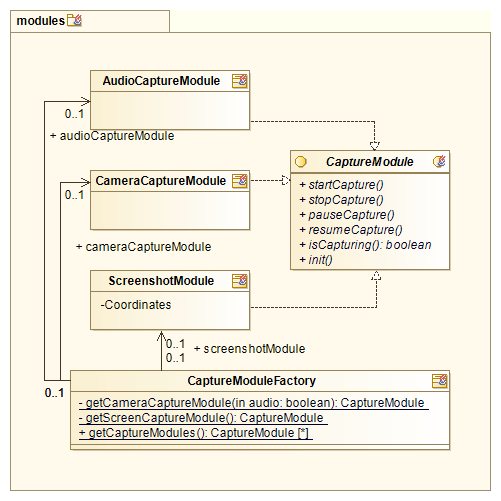
\includegraphics[width=\linewidth]{img/modules_Class_diagram}
\caption{Klassendiagramm des Pakets \mbox{\texttt{modules}}.}
\label{fig:modules_class_diagram}
\end{wrapfigure}
Abbildung \ref{fig:modules_class_diagram} zeigt einige Klassen im Paket \texttt{modules}.
Um die Implementierung der einzelnen \enquote{Module} zu vereinheitlichen gibt es ein Interface \texttt{CaptureModule}, welches die benötigten Methodensignaturen enthält und von den \texttt{*Module} Klassen realisiert wird.
Durch die Vereinheitlichung können die Module in Schleifen durchlaufen gestartet und angehalten werden, unabhängig von der konkreten Klasse.
Die einzelnen Klassen sind als statische Singletons \cite[vgl.][21\psq]{designpattern} implementiert.
Besonders bei Klassen mit exklusivem Hardwarezugriff (\texttt{CameraCaptureModule, AudioCaptureModule}) wird so verhindert, dass mehrere Objekte erstellt werden, was zu Laufzeitfehlern führen könnte.

Das Erzeugen bzw. die Auswahl der Module erfolgt im Sinne des Factory Design Patterns \cite[4-6]{designpattern}.
Dadurch wird erst in der \texttt{CaptureModuleFactory} Klasse entschieden, welche Module instanziert und übergeben werden, abhängig davon, ob ein Root-Zugriff möglich und aktiviert ist und von den aktivierten Modulen.

\subsubsection{Frontkamera und Mikrofon}
Bei der Auswertung von Usability-Tests kann die Mimik der Testperson zur Interpretation beitragen.
Außerdem kann durch das Kamerabild gesehen werden, ob die Testperson sich auf die gestellte Aufgabe konzentriert oder abgelenkt ist.
Dies ist von Bedeutung, wenn der Zeitfaktor bei der Auswertung berücksichtigt wird.
Neben dem Kamerabild werden Sprache und Umgebungsgeräusche mit dem integrierten Mikrofon aufgezeichnet.

Das Aufzeichnen von Bild und Ton erlaubt, neben anderen Testmethoden, auch die \emph{Thinking aloud} Methode (siehe Abschnitt \ref{sec:thinking_aloud});

Die Herausforderung bei der Implementierung stellt sich durch Beschränkungen des Android Betriebssystems.
Dieses sieht vor, dass bei der Aufnahme von Videos und Fotos mit der Kamera eine Vorschau auf dem Bildschirm dargestellt wird.
Dieser soll jedoch vollständig der zu testenden Anwendung zur Verfügung stehen.
Die Lösung besteht darin einen \texttt{SurvaceView} zu erstellen, welcher als System Overlay über allen anderen Bildschirmelementen gezeichnet wird. 
Dieser wird mit einem transparenten Pixelformat versehen, auf 1x1 Pixel verkleinert und in die obere linke Bildschirmecke verschoben.

Somit wird eine, für den Benutzer nicht sichtbare, Vorschau erstellt und die Aufzeichnung kann über die vom System bereitgestellten Klassen erfolgen.


\subsubsection{Bildschirminhalt mit Root-Zugriff}
Mit Root-Zugriff ist das erstellen einzelner Screenshots mit wenigen Zeilen Quelltext möglich, wie in Listing \ref{listing:screenshot_root} dargestellt.

\begin{lstlisting}[label=listing:screenshot_root,language=Java, caption=Screenshot Aufnahme mit Root-Zugriff]
sh = Runtime.getRuntime().exec("su", null, null); // Superuser Rechte holen
OutputStream os = sh.getOutputStream();
os.write("/system/bin/screencap -p /sdcard/outputfile.png"); // Screenshot erstellen
os.flush(); // Schreibpuffer leeren 
os.close(); // und schliessen
sh.waitFor(); // Auf Beendigung der o.g. Befehle warten
\end{lstlisting}

Ab Android~4 wird ein natives Kommandozeilenprogramm \texttt{screencap} mitgeliefert.
Dieses erlaubt das Erstellen von Screenshots, indem direkt der \emph{FrameBuffer} des Systems ausgelesen wird (siehe Quelltext zu \texttt{screencap}\footnote{screencap Quelltext: \url{https://github.com/android/platform_frameworks_base/blob/master/cmds/screencap/screencap.cpp}}).
Der Parameter \texttt{-p} gibt an, dass das Ausgabeformat \texttt{PNG} sein soll. 
Optional kann noch die Nummer des Displays nach dem optionalen Parameter \texttt{-d} angegeben werden.
Am Ende des Aufrufs steht der Pfad der Ausgabedatei, im Beispiel in Zeile 3 \texttt{/sdcard/outputfile.png}. 

Das \emph{Rooting} des Android Betriebssystems wird von diesem selbst nicht verhindert, jedoch muss ggf. der Bootloader entsperrt werden, was zu einer Löschung der Gerätedaten aus Sicherheitsgründen führen kann. 
Neben den Vorteilen, die \emph{Rooting} bietet, wie z.B. erweitertes Debugging oder vollständige Backups, so hat es einige Nachteile oder ist teilweise nicht mit einfachen Möglichkeiten erreichbar \cite[vgl.][]{androidsecurity}.
Um das \emph{Rooting} oder die Installation von alternativen Betriebssystemen oder Versionen zu verhindern verschlüsseln einige Hersteller die Bootloader ihrer Geräte \cite[vgl.][6\psq]{androiddataintegrity}.

Der Vollzugriff auf das Dateisystem und das Betriebssystem kann jedoch auch zu Sicherheitsproblemen führen und daher z.B. in Unternehmen für betrieblich genutzte Geräte untersagt werden.
Demnach kann nicht davon ausgegangen werden, dass nicht immer ein Root-Zugriff möglich ist.

\pagebreak

\subsubsection{Bildschirminhalt ohne Root-Zugriff}
Da ohne Root-Zugriff nicht auf die nativen Anwendungen zugegriffen werden kann, wurde eine alternative Lösung entwickelt.
Die Bibliothek läuft bei der Ausführung der Applikation in deren Kontext und im selben Prozess.
Dadurch ist es möglich auf die Activities der Applikation zuzugreifen.

In Listing \ref{lst:client_screenshot} ist dargestellt, wie ein Bild von einer Activity erstellt wird.
Der direkte Zugriff auf den FrameBuffer oder andere Stationen der Ausgabekette ist nicht möglich, daher wird der Bildschirminhalt \enquote{nachgezeichnet}.
Mit dieser Implementierung werden allerdings nur grafische Elemente der Anwendung erfasst, ein Zugriff auf die Statusleiste, Navigationsleiste oder andere Anwendungen ist so nicht möglich.

\begin{lstlisting}[label=lst:client_screenshot,language=Java, caption=Screenshot Aufnahme ohne Root-Zugriff]
Display display = activity.getWindowManager().getDefaultDisplay();
Point size = new Point();
display.getSize(size);
// RootView holen
View view = activity.getWindow().getDecorView().getRootView();
// Bitmap und Canvas erstellen
Bitmap bitmap = Bitmap.createBitmap(size.x, size.y, Bitmap.Config.ARGB_4444);
Canvas canvas = new Canvas(bitmap);
// Theme holen und anwenden
final Resources.Theme theme = activity.getTheme();
final TypedArray ta = theme.obtainStyledAttributes(new int[]{android.R.attr.windowBackground});
final int res = ta.getResourceId(0, 0);
final Drawable background = activity.getResources().getDrawable(res);
// Hintergrund zeichnen
background.draw(canvas);
// Views zeichnen
view.draw(canvas);
// Bild komprimieren und ins Dateisystem schreiben
FileOutputStream fos = new FileOutputStream("/sdcard/screenshot.png"));
bitmap.compress(Bitmap.CompressFormat.PNG, 90, fos);
fos.flush();
fos.close();
\end{lstlisting}

Das erstellen eines Bildes der Anwendung verläuft in mehreren Schritten.
Über die \texttt{Activity} kann auf den \texttt{WindowManager} und auf das Standarddisplayobjekt zugegriffen werden, um die Bildschirmgröße zu bestimmen.
Danach wird der \texttt{RootView}, der alle anderen grafischen Elemente enthält als Referenz zwischengespeichert.
Zum erstellen des Bildes wird ein \texttt{Bitmap} in Bildschirmgröße erstellt um anschließend ein \texttt{Canvas} Objekt zu erzeugen, auf dem grafische Elemente gezeichnet werden können.
Darauf werden nun nacheinander, beginnend mit dem Hintergrund, die grafischen Elemente gezeichnet.

Abschließend wird das Bild komprimiert und in eine Datei geschrieben.

\pagebreak

\subsubsection{Visualisieren von Benutzereingaben}
Um die Benutzereingaben von einer \texttt{Activity} zu bekommen, wird ein \texttt{View.OnTouchListener} von der Klasse \texttt{ScreenshotModule} implementiert und registriert:
\\
\texttt{activity.getWindow().getDecorView().getRootView().setOnTouchListener(this)}.
Bei einem, durch Benutzereingaben ausgelöstem, \emph{MotionEvent} wird die überschriebene Funktion \texttt{onTouch()} aufgerufen, welcher der auslösende \texttt{View} und das \texttt{MotionEvent} übergeben werden.

Das \texttt{MotionEvent} wird auf zwei konstante Integer-Werte geprüft. 
\texttt{ACTION\_MOVE} beschreibt einen Teil einer Geste und \texttt{ACTION\_UP} beschreibt deren Ende.
Die Koordinaten der \emph{MotionEvents} werden so lange gesammelt, wie die Geste andauert, und danach an die Methode \texttt{takeScreenshot} übergeben, in welcher diese zusätzlich auf das \texttt{Canvas} Objekt, als rote Punkte,  gezeichnet werden.



\subsection{Benutzeroberfläche}
\begin{minipage}[t]{0.45\linewidth}
	\centering
	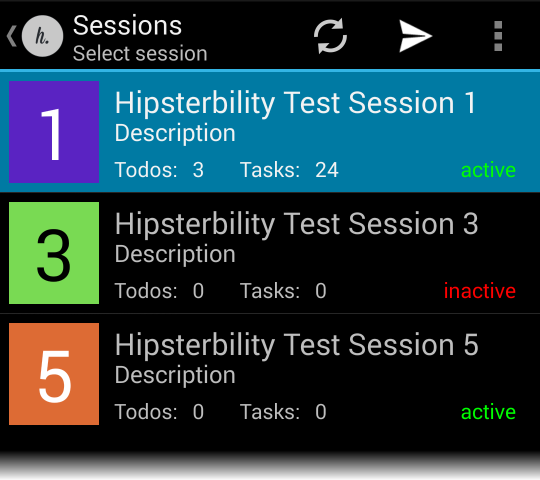
\includegraphics[width=\linewidth]{img/screen_session_list}
	\captionof{figure}{SessionActivity Screenshot} \label{fig:screen_sessions}
\end{minipage}
\hfill
\begin{minipage}[t]{0.45\linewidth}
	\centering
	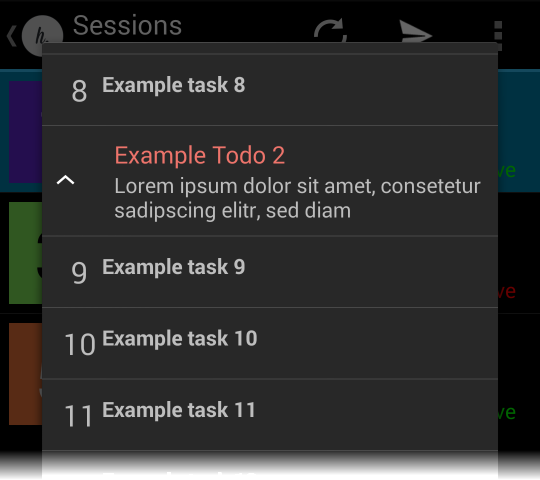
\includegraphics[width=\linewidth]{img/screen_todos_tasks}
	\captionof{figure}{TodosActivity Screenshot} \label{fig:screen_todos_tasks}
\end{minipage}

% Figure verschoben
\pagebreak

\begin{wrapfigure}[33]{l}{0.45\textwidth}
	\centering
	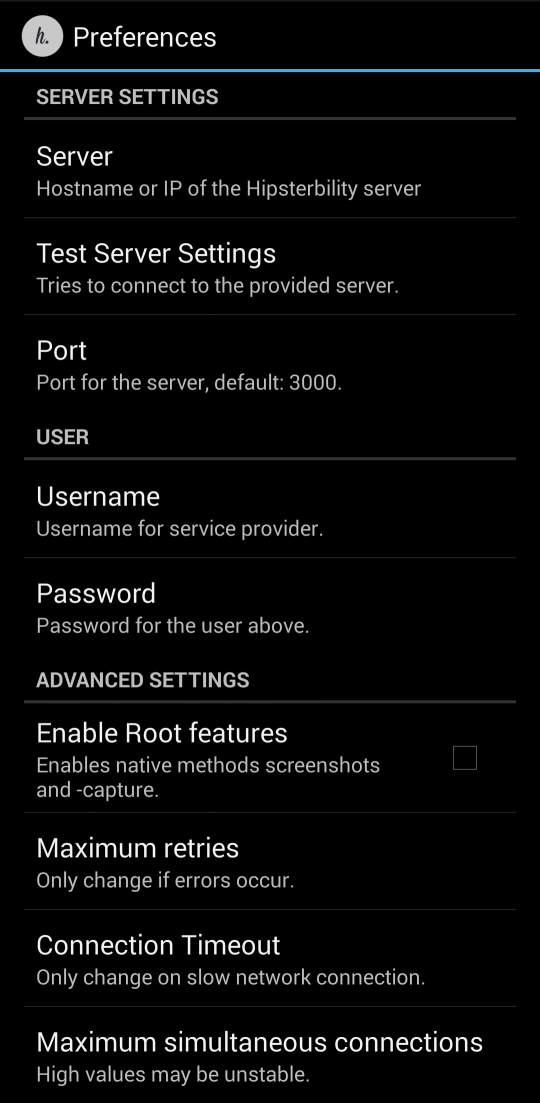
\includegraphics[width=\linewidth]{img/screen_settings}
	\captionof{figure}{SettingsActivity Screenshot} \label{fig:screen_settings}
	\vspace{-35mm}
\end{wrapfigure}

Aus den Anforderungen geht hervor, dass Testpersonen eine Session aussuchen, sich die zugehörigen Todos und Tasks ansehen und diese bearbeiten, wobei entsprechende Daten erfasst werden.
Außerdem ist es sinnvoll, Einstellungen vornehmen zu können (Serveradresse, Port etc.). Auch die Daten für die Benutzerauthentifizierung sollten aus der Applikation heraus anpassbar sein.
Um diese Anforderungen umzusetzen wurden drei Activities erstellt, jeweils zum Anzeigen und Auswählen der Sessions (Abbildung \ref{fig:screen_sessions}, für die Anzeige von Todos und Tasks (Abbildung \ref{fig:screen_todos_tasks}) sowie eine weitere für Einstellungen und Optionen (Abbildung \ref{fig:screen_settings}), welche aus dem Menü der SessionActivity heraus gestartet werden kann.


Ein Großteil der Implementierung sind Services.
Sie laufen im Hintergrund, meist unabhängig von der jeweiligen Vordergrund-Activitiy.
Diese Entkopplung von Benutzeroberfläche und Programmlogik ist besonders nützlich, da Daten über die Interaktion mit \emph{Activities} gesammelt werden, die nicht zur Bibliothek gehören.
Diese Hintergrunddienste können beispielsweise über Intents gesteuert werden, welche von jeder Komponente gesendet werden können, die über einen \texttt{Context} verfügt.
Dazu zählen \emph{Activites}, \emph{Services}, \emph{Applications} und jede Klasse, die aus einem Objekt der zuvor genannten den \emph{Context} mittels \texttt{getApplicationContext()} holt.
Außerdem können \emph{Intents} auch aus \emph{Notifications} gestartet werden, indem sie in \emph{PendigIntents} an diese übergeben werden.
Dieses Prinzip hat den Vorteil, dass eine Steuerung von Hintergrunddiensten möglich ist, ohne der Activity im Vordergrund den Fokus zu nehmen.
Dieser Ansatz wurde für die Implementierung gewählt, da die Bibliothek so weitgehend im Hintergrund arbeitet, bei Bedarf jedoch Informationen an den Benutzer weitergegeben und Aktionen ausgelöst werden können.

Abbildung \ref{fig:notification_main} zeigt die Benachrichtigung, welche beim Aktivieren der Bibliothek angezeigt wird. 
Damit sie nicht versehentlich durch eine Wischgeste entfernt wird, erfolgt das Anzeigen mit der Service-Methode \texttt{startForegroud()}.
Das Berühren der ausklappbaren Schaltfläche \emph{Dismiss} führt zum Entfernen der Benachrichtigung und dem Beenden des Hintergrunddienstes.
Die Bibliothek wird dadurch inaktiv, bis die Applikation das nächste Mal gestartet wird.

\begin{minipage}[t]{0.45\linewidth}
	\centering
	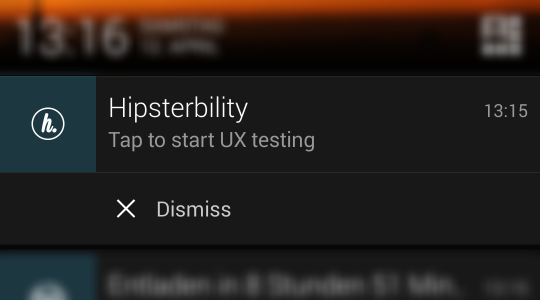
\includegraphics[width=\linewidth]{img/notification_main}
	\captionof{figure}{Notification zum Starten der Bibliothek (Screenshot)} \label{fig:notification_main}
\end{minipage}
\hfill
\begin{minipage}[t]{0.45\linewidth}
	\centering
	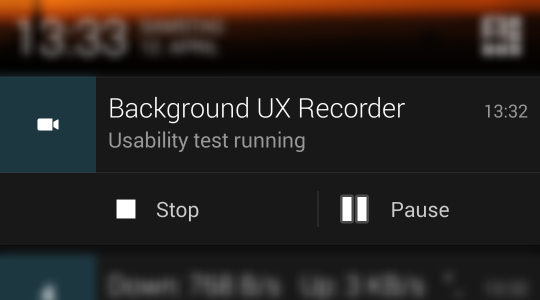
\includegraphics[width=\linewidth]{img/notification_background_recorder}
	\captionof{figure}{Notification bei laufender Datenerfassung (Screenshot)} \label{fig:notification_recorder}
\end{minipage}


Abbildung \ref{fig:notification_recorder} zeigt die Benachrichtigung, welche während der Datenerfassung angezeigt wird.
Zusätzlich werden beim Start der Aufzeichnung des Kamerabildes die Standard-Töne des Betriebssystems für die Kamera abgespielt.
Um die Testperson weiterhin dauerhaft über die laufende Datenerfassung zu informieren wird zusätzlich ein Icon (\texttt{ImageView}) dauerhaft im Vordergrund angezeigt, welches unabhängig von der laufenden \texttt{Activity} ist (Abbildung \ref{fig:icon_record_on_top}).

Auch sie kann nicht durch eine Wischgeste entfernt werden und bietet die Möglichkeiten die Datensammlung zu unterbrechen (\emph{Pause}) oder zu Beenden (\emph{Stop}), worauf die Benachrichtigung zum Hochladen der Daten zum Server angezeigt wird (Abbildung \ref{fig:notification_upload_data}).
Wird diese durch eine Berührung aktiviert, startet das Hochladen der gesammelten Daten zum Server und dessen Fortschritt wird angezeigt (Abbildung \ref{fig:notification_upload_progress}).
Wenn das Hochladen abgeschlossen ist, können die gesammelten Daten vom Gerät gelöscht werden (siehe Abbildung \ref{fig:notification_upload_finished}).

Im Fall eines Fehlers wird dieser dem Benutzer entweder durch ein \texttt{Toast} oder durch einen \texttt{AlertDialog} angezeigt, abhängig von der Situation.

\begin{minipage}[t]{0.45\linewidth}
	\centering
	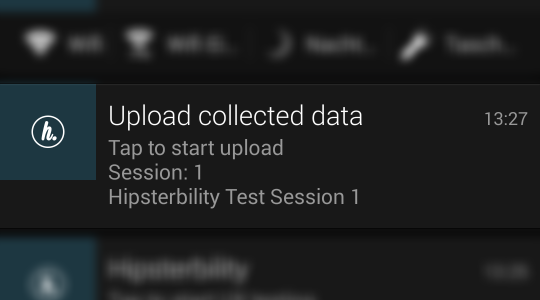
\includegraphics[width=\linewidth]{img/notification_upload_data}
	\captionof{figure}{Notification zum Hochladen der Daten (Screenshot)} \label{fig:notification_upload_data}
\end{minipage}
\hfill
\begin{minipage}[t]{0.45\linewidth}
	\centering
	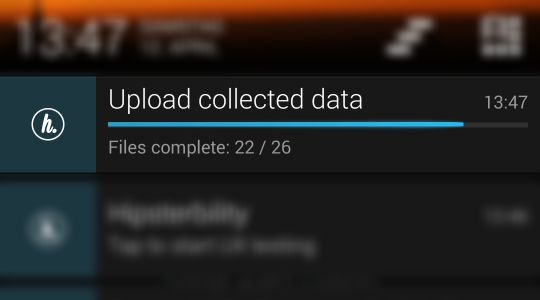
\includegraphics[width=\linewidth]{img/notification_upload_progress}
	\captionof{figure}{Notification bei laufendem Hochladen von Daten (Screenshot)} \label{fig:notification_upload_progress}
\end{minipage}

\begin{minipage}[t]{0.45\linewidth}
	\centering
	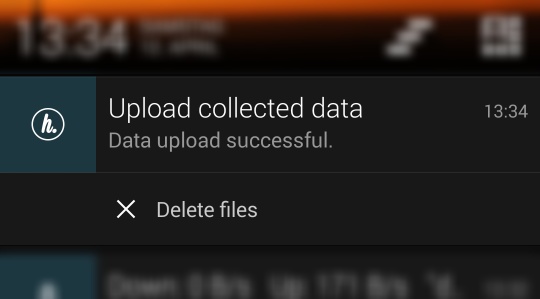
\includegraphics[width=\linewidth]{img/notification_upload_finished}
	\captionof{figure}{Notification für vollständigen Upload (Screenshot)} \label{fig:notification_upload_finished}
\end{minipage}
\hfill
\begin{minipage}[t]{0.45\linewidth}
	\centering
	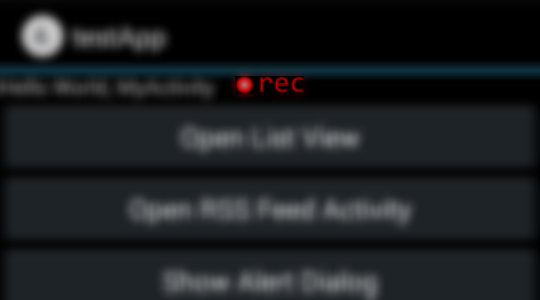
\includegraphics[width=\linewidth]{img/record_on_top_icon}
	\captionof{figure}{Overlay Icon bei laufender Datenerfassung (Screenshot)} \label{fig:icon_record_on_top}
\end{minipage}

\subsection{Einbinden der Bibliothek in eigene Anwendungen}
Die Bibliothek kann auf zwei Arten in bestehende -- und neue -- Projekte eingebunden werden.
Zum einen kann sie als zusätzliches Modul hinzugefügt werden (\textbf{File | Import Module...}), wobei zu beachten ist, dass in den Moduleinstellungen (\textbf{File | Project Structure...}), nach dem Import, der Haken \texttt{Library module} gesetzt ist (siehe Abbildung \ref{fig:screen_intellij_library_module} im Anhang \ref{apdx:intellij}).


Auch die Einstellungen für die zu testende Applikation sollten ggf. angepasst werden, da die Bibliothek eine eigene \texttt{AndroidManifest.xml} Datei mitbringt.
Das aktivieren des Zusammenfügens der Maifeste (Abbildung \ref{fig:screen_intellij_maifest_merging} im Anhang \ref{apdx:intellij}) sorgt für ein automatisches Zusammenfassen der verschiedenen Manifest-Dateien.



Die Bibliothek benötigt für eine korrekte Ausführung die folgenden \emph{Permissions}\footnote{Android Permissions: \url{http://developer.android.com/guide/topics/security/permissions.html}}\\ (\texttt{android.permission.*}):

\begin{description}
	\item[\texttt{WRITE\_EXTERNAL\_STORAGE}]
		Dateien in den Massenspeicher schreiben.
	\item[\texttt{RECORD\_AUDIO}]
		Aufzeichnung von Ton mittels des integrierten Mikrofons.
	\item[\texttt{CAMERA}]
		Zugriff auf die Frontkamera.
	\item[\texttt{SYSTEM\_ALERT\_WINDOW}]
		Icon für das Signalisieren der laufenden Datenerfassung.
	\item[\texttt{ACCESS\_SUPERUSER}]
		Root-Zugriff (falls verfügbar).
	\item[\texttt{INTERNET}]
		Netzwerkzugriff (mobil und lokal).
\end{description}

Außerdem müssen die \emph{Services} und \emph{Activities} im System registriert werden, damit diese mit \emph{Intents} gestartet werden können. Die vollständige Manifest-Datei befindet sich im Anhang \ref{apdx:manifest} (Listing \ref{lst:androidmanifest}).


\subsubsection{Dynamisches Einbinden - Pre-Dexing}
Beim Pre-Dexing können mehrere Android-Projekte zu einem Projekt hinzugefügt werden. 
Da die Bibliothek neueste Funktionen des Android-Betriebssystems verwendet, muss auf dem  Gerät zur Kompilierung einer Anwendung aktuelle Build-Tools der Android-SDK vorliegen.
Im Falle der Bibliothek ist dies API-Level 19. Offenbar hat sich hier ein Bug eingeschlichen und es ist unter der Version 19.0 kein Pre-Dexing möglich.
Dies wurde allerdings bereits behoben. Es sei gesagt, dass mindestens die Version 19.0.1 verwendet werden muss um Pre-Dexing durchführen zu können.


\subsubsection{Statisches Einbinden als JAR-Archiv}
Über \textbf{FILE | Project Structure | Artifacts} kann in \emph{IntelliJ} die Bibliothek als \ac{JAR}-Archiv exportiert werden.
Um diese in ein anderes Projekt einzubinden wird das Archiv in den \texttt{libs} Unterordner kopiert (ggf. muss der Ordner erstellt werden) und über \textbf{Rechtsklick auf das JAR-Archiv in der IntelliJ Projektstruktur | Add as Library...} als Bibliothek hinzugefügt werden.
In der IntelliJ Online Hilfe\footnote{IntelliJ -- Configuring Module Dependencies and Libraries:  \url{http://www.jetbrains.com/idea/webhelp/configuring-module-dependencies-and-libraries.html}} ist eine ausführlichere Beschreibung zu finden.

\subsection{Bekannte Einschränkungen}
Der gegenwärtige Stand der Bibliothek enthält einige Einschränkungen bei der Nutzung. 
Einerseits sind die Aufnahme von Videos und Screenshots, basierend auf nativen Funktionen mit Root-Zugriff zwar implementiert und getestet, allerdings nicht vollständig in den Gesamtablauf eingebunden und können entsprechend nicht beim Testen von Applikationen genutzt werden.
Auch der Wechsel von Activities wird aktuell noch nicht voll unterstützt.
Wenn keine Activity der Testanwendung mehr im Vordergrund ist wird zwar die Aufnahme nach einem Timeout gestoppt, beim Wechsel in eine andere Activty der Testapplikation wird diese nicht weiter aufgezeichnet.
Nur die Video- und Audioaufzeichnung im Hintergrund wird fortgesetzt, der Bildschirminhalt wird nicht weiter aufgezeichnet.

Weiterhin werden -- nicht-bildschirmfüllende -- Elemente wie Dialoge, Benachrichtigungen und Toasts bei der Bildschirmaufzeichnung nicht erfasst, da i.d.R. über Systemdienste erstellt werden.

Auch der Ablauf von Tasks und Todos lässt sich im aktuellen Stand nicht nachverfolgen.
Außerdem hat die Testperson aktuell keine Möglichkeit sich -- nach dem Start einer Session -- noch einmal die Aufgabenstellung anzusehen.

Eine weitere Hürde stellt der Orientierungswechsel des Geräts während der Datenerfassung dar, da die Orientierung des Kamerabildes nur beim starten der Aufnahme bestimmt wird.
Das erstellen von Screenshots funktioniert zwar weiterhin, allerdings nicht das native Screen Recording.
Bei diesem würde ein Teil des Bildbereichs abgeschnitten und schwarze Balken eingefügt.
 
 
\subsection{Ausblick und Weiterentwicklung}
\label{sec:client_offene_punkte}
\subsubsection{Application Lifecycle}
Neben den Interaktionen des Benutzers mit einzelnen Activities oder Bildschirmelementen kann auch eine Auswertung des Lebenszyklus der Applikation und enthaltener Activities Aufschlüsse liefern.
So kann beispielsweise durch das (automatische) statistische Auswerten von entsprechenden Logdateien analysiert werden, in welcher Häufigkeit und Reihenfolge Activities aufgerufen werden, oder ob einzelne gar nicht gestartet werden, weil z.B. ein Button nicht funktioniert oder Testpersonen die Funktion nicht finden.

\subsubsection{Protokollierung von Benutzereingaben}
Auch wenn Benutzereingaben auf den Aufnahmen vom Bildschirminhalt visualisiert werden, kann eine zusätzliche Protokollierung in maschinenlesbaren weitere (automatisierte) Analysemöglichkeiten bieten.
Anhand von statistischen Analysen kann z.B. herausgefunden werden, dass Testpersonen Reaktionen auf Gesten erwarten, die nicht implementiert wurden.
Zusätzlich können Zeitabstände zwischen einzelnen Eingaben ausgewertet und interpretiert werden, um herauszufinden wie leicht verständlich Benutzeroberflächen durch Testpersonen wahrgenommen werden.

\subsubsection{Benutzeroberfläche und Interaktion}
Bisher werden Testpersonen nur wenig Möglichkeiten geboten Aufgaben nachzuverfolgen oder nachzuschlagen.
Beim Start einer Session werden diese Angezeigt, können aktuell, im Verlauf der Datenerfassung, allerdings nicht noch einmal aufgerufen werden.
Auch das Layout und Design der Benutzeroberfläche können weiter verbessert werden.
Einige Symbole dienen nur als Platzhalter können gegen passendere ersetzt werden.
Bisher wurden Layout und Design einzig für Smartphones optimiert, sie funktionieren schlecht auch auf Tablets, da nur wenige Informationen auf einen deutlich größeren Bildschirm dargestellt werden.

\subsubsection{Sicherheit}
Die Kommunikation mit dem Server verläuft unverschlüsselt mittels \ac{HTTP}-Methoden.
Auch Benutzername und Passwort werden aktuell unverschlüsselt im Klartext übertragen und können einfach Mitgelesen werden.
Die Speicherung des Passworts auf dem Endgerät erfolgt durch das Android Pereferences Framework in unverschlüsselten Textdateien und kann mit Root-Zugriff leicht ausgelesen werden.  
Um die Kommunikation sicherer zu gestalten sollte die Kommunikation verschlüsselt werden, z.B. mittels \ac{SSL} bzw. \ac{TLS}, da das Android Betriebssystem Bibliotheken für diese Verfahren mitbringt.
Zur sichereren Speicherung von Benutzername und Passwort könnte z.B. die Android interne Kontenverwaltung genutzt werden.

\subsubsection{Kommunikation}
Bisher werden Sessions, Todos und Tasks beim Starten der Bibliothek vom Server abgerufen und nicht lokal zwischengespeichert. 
Zwischen dem Starten der Aufzeichnung und dem Hochladen der gesammelten Daten wird keine Verbindung zum Server hergestellt.
Denkbar wäre eine Zwischenspeicherung der Daten für den Offline Einsatz.
Dieser Ansatz würde auch Tests außerhalb der Laborumgebung ermöglichen.

\pagebreak

\section{Messdaten}

\pagebreak

\section{Ergebnis}
\pagebreak

\section{Offene Punkte}

% More content goes here

\thispagestyle{empty}

%\renewcommand*{\biburlprefix}{(URL: }
%\renewcommand*{\biburlsuffix}{)}

\pagebreak
\addcontentsline{toc}{section}{Literaturverzeichnis} % Eintrag ins Inhaltsverzeichnis
\printbibliography

\pagebreak
\appendix
\addcontentsline{toc}{section}{Anhänge}

\end{document}
	
